\chapter{Channel flow} \label{chap:chanFlow}
\renewcommand{\tabdir}{chapters/part_processes/channelFlow/tab}
\renewcommand{\figdir}{chapters/part_processes/channelFlow/fig}

\section{Introduction} \label{sec:chanFlow_intro}

This chapter desribes approaches to the simulation of open channel flow. In a dynamic model, we generally deal with unsteady flow conditions. One can distinguish between two basic concepts:

\begin{description}
  \item[Hydrodynamic approach] Such models are based on a solution of the St. Venant equations, expressing the conservation of momentum and mass. The solution of these (possibly simplified) partial differential equations requires rather expensive numerical methods.
  \item[Hydrological approaches] Such models still consider the principle of mass conservation (continuity equation). However, in contrast to hydrodynamic models, they do not account for the conservation of momentum or energy but rely on empirical relations between channel storage and flow.
\end{description}

In hydrological catchment models, hydrological approaches are widely because they are easier to implement and allow for fast computations based on anaytical solutions. Prominent examples include:
\begin{itemize}
  \item the single reservoir approach,
  \item the Muskingum method,
  \item the method of Kalinin-Miljukov (Nash's cascade).
\end{itemize}

The approach(es) described below apply to a single reach. Here, a reach is defined as a river section of a constant geometry (\ie{} cross-section and slope). In hydrological catchment modeling for larger areas, cross-section and slope data are usually scarce and a constant geometry is therefore assumed between the neighbored junctions along a river. Then, a reach is practically identical to the river section between two junctions.

%%%%%%%%%%%%%%%%%%%%%%%%%%%%%%%%%%%%%%%%%%%%%%%%%%%%%%%%%%%%%%%%%%%%%%%%%%%%%%%%
%%%%%%%%%%%%%%%%%%%%%%%%%%%%%%%%%%%%%%%%%%%%%%%%%%%%%%%%%%%%%%%%%%%%%%%%%%%%%%%%
%%%%%%%%%%%%%%%%%%%%%%%%%%%%%%%%%%%%%%%%%%%%%%%%%%%%%%%%%%%%%%%%%%%%%%%%%%%%%%%%

\section{Single reservoir approach} \label{sec:chanFlow_singleRes}

%%%%%%%%%%%%%%%%%%%%%%%%%%%%%%%%%%%%%%%%%%%%%%%%%%%%%%%%%%%%%%%%%%%%%%%%%%%%%%%%

\subsection{Processes and equations} \label{sec:chanFlow_singleRes_processes}

In this approach, a reach (\figref{fig:chanFlow_singleRes_reach}) is treated as a single reservoir. Considering the principle of mass conservation, the storage volume $v$ (\cbm) is related to the rates of inflow $q_{in}$ and outflow $q_{out}$ (both in \cbm/s) by the continuity equation \eqnref{eqn:chanFlow_singleRes_continuity_QinConst}.

\begin{equation} \label{eqn:chanFlow_singleRes_continuity_QinConst}
  \frac{dv}{dt} = q_{in} - q_{out}
\end{equation}

\begin{figure}
  \centering
  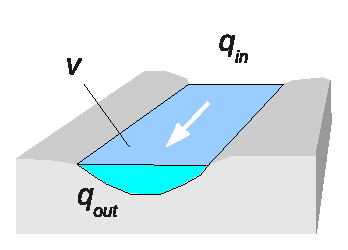
\includegraphics[width=0.6\columnwidth]{\figdir/reach.eps}
  \caption{Sketch of a reach with storage volume $v$, and the rates of in- and outflow ($q_{in}$, $q_{out}$). \label{fig:chanFlow_singleRes_reach}}
\end{figure}

To simulated the dynamics of $v$ for a given inflow rate, the continuity equation must be complemented by a second equation relating $q_{out}$ to $v$. In the case of a linear reservoir, for example, this missing relation is given by \eqnref{eqn:chanFlow_singleRes_outflowLinear} where $k$ is a retention constant with the dimension of a time. The advantage of this linear relation is that it allows for an analytical solution of \eqnref{eqn:chanFlow_singleRes_continuity_QinConst}.

\begin{equation} \label{eqn:chanFlow_singleRes_outflowLinear}
  q_{out}= \frac{1}{k} \cdot v
\end{equation}

Assuming that the inflow rate $q_{in}$ is constant over a discrete time step of length $\Delta t$, combining \eqnref{eqn:chanFlow_singleRes_continuity_QinConst} and \ref{eqn:chanFlow_singleRes_outflowLinear} and subsequent integration using the substitution method yields \eqnref{eqn:chanFlow_singleRes_linResSolution_QinConst}.

\begin{equation} \label{eqn:chanFlow_singleRes_linResSolution_QinConst}
  v(t_0 + \Delta t) =  (v(t_0) - q_{in} \cdot k) \cdot e^{(-\Delta t / k)} + q_{in} \cdot k
\end{equation}
\medskip
\begin{tabular}{lll}
  $v(t_0)$ & Initial storage at & L$^3$ \\
  $\Delta t$ & Length of time step & T \\
\end{tabular}

A slightly advanced version of the linear reservoir model is obtained if the inflow rate $q_{in}$ is allowed to vary linearly with time. Then, the modified continuity equation is given by \eqnref{eqn:chanFlow_singleRes_continuity_QinLinear}

\begin{equation} \label{eqn:chanFlow_singleRes_continuity_QinLinear}
  \frac{dv}{dt} = q_{in,0} + (q_{in,1} - q_{in,0}) \cdot t - q_{out}
\end{equation}

where $q_{in,0}$ and $q_{in,1}$ represent an initial and final inflow rate, respectively. After combining \eqnref{eqn:chanFlow_singleRes_continuity_QinLinear} with \eqnref{eqn:chanFlow_singleRes_outflowLinear}, the integration yields \eqnref{eqn:chanFlow_singleRes_linResSolution_QinLinear}

\begin{align} \label{eqn:chanFlow_singleRes_linResSolution_QinLinear}
  v(t_0 + \Delta t) =  & v(t_0) \cdot x + \frac{a \cdot (x-1)}{b^2} \\
                       & + \frac{q_{in,0} \cdot (x-1) - a \cdot \Delta t}{b} \nonumber
\end{align}

with the abbreviations

\begin{align*}
  a= & (q_{in,1} - q_{in,0}) / \Delta t \\ \nonumber
  b= & -1/k \\ \nonumber
  x= & e^{(-\Delta t / k)} \nonumber
\end{align*}

and

\begin{align*}
  q_{in,0} = q_{in}(t_0) \\ \nonumber
  q_{in,1} = q_{in}(t_0 + \Delta t) \nonumber
\end{align*}

This equation is also used in the LARSIM model \citep[same as Equation 3.54 in][]{Ludwig2006}.

Unfortunately, for natural channels, the relation between $q_{out}$ and $v$ is typically non-linear and  \eqnref{eqn:chanFlow_singleRes_outflowLinear} is therefor not applicable. However, the analytical solution of the linear reservoir equation (\eqnsref{eqn:chanFlow_singleRes_linResSolution_QinConst} or \ref{eqn:chanFlow_singleRes_linResSolution_QinLinear}) is very attractive to use because of its low computational cost. A common solution to this problem is the idea of a locally-linear reservoir. In this concept, the analytical solution of the linear reservoir equation is still used but the retention constant $k$ is allowed to depend on the storage volume $v$ (or the outflow rate $q_{out}$).

According to \eqnref{eqn:chanFlow_singleRes_outflowLinear}, the retention constant of a linear reservoir is given by \eqnref{eqn:chanFlow_singleRes_retConst_trueLinear}

\begin{equation} \label{eqn:chanFlow_singleRes_retConst_trueLinear}
 k = \frac{v}{q_{out}}
\end{equation}
.

Similarly, for the locally-linear reservoir, the retention constant is given by \eqnref{eqn:chanFlow_singleRes_retConst_locallyLinear}

\begin{equation} \label{eqn:chanFlow_singleRes_retConst_locallyLinear}
 k = \frac{\Delta v}{\Delta q_{out}}
\end{equation}
.

Thus, the retention constant $k$ still equals the slope of the relation between $v$ and $q_{out}$  (\figref{fig:chanFlow_singleRes_dVdQ}).

\begin{figure}
  \centering
  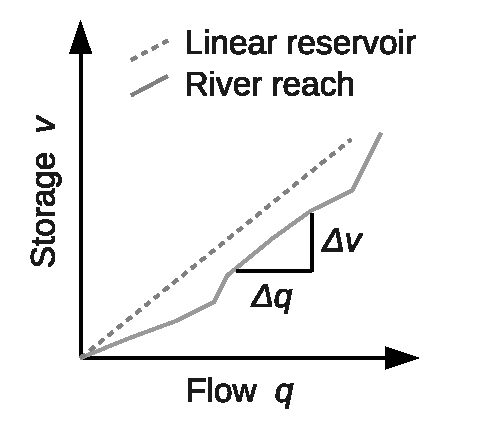
\includegraphics[width=0.5\columnwidth]{\figdir/dVdQ.eps}
  \caption{Relation between storage volume $v$ and outflow rate $q_{out}$ for a linear reservoir and a river reach. \label{fig:chanFlow_singleRes_dVdQ}}
\end{figure}

For channels of known geometry, the relation between $q_{out}$ to $v$ (\figref{fig:chanFlow_singleRes_dVdQ}) can be derived from a rating curve, \ie{} corresponding observations of flow rates and water levels (the latter being convertable to storage volumes). Since the vast majority of simulated reaches in a hydrological model is ungaged, rating curves are not practically available and need to be estimated. This is usually done by applying Manning's equation (\eqnref{eqn:chanFlow_singleRes_manning}).

\begin{equation} \label{eqn:chanFlow_singleRes_manning}
  q(h)= \frac{1}{n} \cdot \sqrt{S_f} \cdot R(h)^{2/3} \cdot A(h)
\end{equation}
\medskip
\begin{tabular}{lll}
  $q$ & Flow rate & \cbm/s \\
  $S_f$ & Slope of the energy grade line & -- \\
  $R$ & Hydraulic radius &  m \\
  $A$ & Wet cross-section area & \sqm \\
  $h$ & Water level & m \\
  $n$ & Manning's $n$ (parameter) & Non-physical \\
\end{tabular}

Considering that the storage volume $v$ in a uniform reach equals $A \cdot L$ ($L$: length of the channel), \eqnref{eqn:chanFlow_singleRes_manning} can be used to tabulate corresponding pairs of $v$ and $q_{out}$ and thus also $k(q_{out})$ or $k(v)$, respectively (recall \eqnref{eqn:chanFlow_singleRes_retConst_locallyLinear}). The required information are:
\begin{itemize}
  \item The functions $A(h)$ and $R(h)$. They can easily be computed from the x-section's geometry (table of offsets and corresponding elevations).
  \item The roughness parameter $n$. Tables and empirical formulas exist to estimate this value from channel properties. It can also be fitted by steady flow modeling.
  \item The slope of the energy grade line $S_f$. In practice, only the slope of the channel bottom $S_0$ is constant and known. It can be measured in the field or has to be gathered from a digital elevation model (with subsequent quality checks).
\end{itemize}

%%%%%%%%%%%%%%%%%%%%%%%%%%%%%%%%%%%%%%%%%%%%%%%%%%%%%%%%%%%%%%%%%%%%%%%%%%%%%%%%

\subsection{Mathematical solution} \label{sec:chanFlow_singleRes_solution}

\subsubsection*{Governing equation}

In each time step, the storage $v$ is updated using \eqnref{eqn:chanFlow_singleRes_linResSolution_QinLinear}. The applied retention constant is an average value ($\overline{k}$) taking into account the initial storage volume, the initial inflow rate, and the inflow rate at the end of the time step (\eqnref{eqn:chanFlow_singleRes_averageK})

\begin{equation} \label{eqn:chanFlow_singleRes_averageK}
  \overline{k} = \frac{k(q_{in}(t_0)) + k(q_{in}(t_0 + \Delta t)) + k(v(t_0))}{3}
\end{equation}

with all $k$ values taken from the $\Delta v/\Delta q$ relation (\eqnref{eqn:chanFlow_singleRes_retConst_locallyLinear}).

To apply \eqnsref{eqn:chanFlow_singleRes_linResSolution_QinLinear} and \ref{eqn:chanFlow_singleRes_averageK}, the inflow rates corresponding to the begin and the end of a time step, $q_{in}(t_0)$ and $q_{in}(t_0 + \Delta t)$, must be known.

\subsubsection*{Inflow rates}

Problems with conservation of mass may arise from using $q_{in}(t_0)$ and $q_{in}(t_0 + \Delta t)$ together with the assumption of a linear variation over $\Delta t$ when simulating multiple reaches in series. This is due to the fact that the outflow from a reach -- and thus the inflow of the downstream reach -- varies exponentially rather than linearly (see \eqnref{eqn:chanFlow_singleRes_linResSolution_QinConst} \& \ref{eqn:chanFlow_singleRes_linResSolution_QinLinear}). To allow for a proper mass balance (priority) while also taking into account the variation in the inflow rate (secondary objective), the model uses as input
\begin{enumerate}
  \item the rate at the end of the time step, $q_{in}(t_0 + \Delta t)$.
  \item the average inflow rate for the time step, $\overline{q_{in}}$.
\end{enumerate}

Then, the inflow rate at the begin of the time step, $q_{in}(t_0)$ is estimated from these two values using
\begin{equation*}
q_{in}(t_0)= max(0., 2 \cdot \overline{q_{in}} - q_{in}(t_0 + \Delta t))
\end{equation*}
and subsequently applying the correction
\begin{equation*}
q_{in}(t_0 + \Delta t)= 2 \cdot \overline{q_{in}} - q_{in}(t_0)
\end{equation*}
The latter correction is necessary to account for the mass balance in those cases where the \second{} argument of $max()$ is negative and $q_{in}(t_0)$ is therefor set to zero. These are cases where the value of the average inflow rate is incompatible with the assumption of a linear variation over $\Delta t$.

\subsubsection*{Outflow rates}

Using the concept of the linear reservoir, the outflow rate at the end of the time step is computed from \eqnref{eqn:chanFlow_singleRes_outflowEnd}.

\begin{equation} \label{eqn:chanFlow_singleRes_outflowEnd}
  q_{out}(t_0 + \Delta t)= \frac{1}{\overline{k}} \cdot v(t_0 + \Delta t)
\end{equation}

The time-step averaged outflow rate is calculated using \eqnref{eqn:chanFlow_singleRes_outflowAvg}, which is a discrete version of the mass balance equation.

\begin{equation} \label{eqn:chanFlow_singleRes_outflowAvg}
\overline{q_{out}}= \frac{v(t_0) - v(t_0 + \Delta t)}{\Delta t} + \overline{q_{in}}
\end{equation}

%%%%%%%%%%%%%%%%%%%%%%%%%%%%%%%%%%%%%%%%%%%%%%%%%%%%%%%%%%%%%%%%%%%%%%%%%%%%%%%%

\subsection{Hints for application} \label{sec:chanFlow_singleRes_hints}

In hydrological catchment modeling, data on the geometry of river cross-sections are usually scarce. The \software{topocatch} software \citep{Echse-Tools-Doc} contains methods to estimate the x-section characteristics for all reaches in a river basin using survey data from a limited number of sites only. Basically, these methods perform a spatial regionalization of the functions $A(h)$ and $R(h)$. It then applies \eqnref{eqn:chanFlow_singleRes_manning} to generate a table of corresponding storage volumes and outflow rates, allowing for look-up of the retention constant (\eqnref{eqn:chanFlow_singleRes_retConst_locallyLinear}).
